\documentclass[12pt]{extarticle}
\usepackage{tempora}
\usepackage[T1, T2A]{fontenc}
\usepackage[utf8]{inputenc}
\usepackage[english, ukrainian]{babel}
\usepackage{geometry}
\usepackage{graphicx}
\usepackage{multirow}
\usepackage{multicol}
\usepackage{float}
\graphicspath{{/home/artem/Pictures}}
\geometry
{
    a4paper,
    left=30mm,
    top=15mm,
    right=20mm,
    bottom=15mm,
}

\begin{document}
\begin{titlepage}
    \begin{center}
        \textbf{\normalsize{\MakeUppercase{
            Міністерство Освіти і науки України
            Національний університет "Львівська політехніка"
        }}}

        \begin{flushright}
        \textbf{ІКНІ}\\
        Кафедра \textbf{ПЗ}
        \end{flushright}
        \vspace{15mm}

        \includegraphics[width=0.4\textwidth]{lpnu_logo.png}

        \vspace*{\fill}

        \textbf{\normalsize{\MakeUppercase{Звіт}}}
            
        До лабораторної роботи №8

        \textbf{на тему:} “НЕЛІНІЙНІ СТРУКТУРИ ДАНИХ: БІНАРНІ ДЕРЕВА”

        \textbf{з дисципліни:} "Алгоритми і структури даних”
            
        \vspace*{\fill}

        \begin{flushright}

            \textbf{Лектор:}\\
            доцент кафедри ПЗ\\
            Коротєєва Т. О.\\
            \vspace{12pt}

            \textbf{Виконав:}\\
            студент групи ПЗ-24\\
            Губик А. С.\\
            \vspace{12pt}

            \textbf{Прийняв:}\\
            асистент кафедри ПЗ\\
            Вишневський К. О.\\
        \vspace{12pt}
        \end{flushright}

        Львів -- 2023
            
            
    \end{center}
\end{titlepage}

\subsection*{Тема роботи} 
НЕЛІНІЙНІ СТРУКТУРИ ДАНИХ: БІНАРНІ ДЕРЕВА

\subsection*{Мета роботи} Oзнайомитися з бінарними деревами та отримати навички програмування алгоритмів, що їх обробляють.


\subsection*{Індивідуальне завдання}
Варіант 3: N  -- символи; змішаний обхід; третій голосний елемент. 



\subsection*{Теоретичні відомості}
Бінарним називають таке 2-арне дерево, в якого один потомок є лівим, а другий - правим. Вершина бінарного дерева може взагалі не мати потомків, або мати тільки ліве, або тільки праве піддерево, або обидва піддерева одночасно.

Рівнем або рангом вершини по відношенню до дерева називають довжину шляху від кореня до цієї вершини. Довжина шляху - це кількість дуг, які треба пройти від кореня для досягнення даної вершини.

Висота дерева дорівнює кількості рівнів у дереві.

Бінарне дерево з m вершинами називають збалансованим, якщо різниця між рівнями будь-яких двох вершин не більша від одиниці.

Алгоритми обходу дерева

Алгоритм обходу дерева являє собою спосіб методичного дослідження вершин дерева, при якому кожна вершина проглядається тільки один раз. Повне проходження дерева дає лінійне розміщення вершин, після якого можна говорите про "наступну вершину" як таку, що розміщується або перед даною вершиною, або після неї. Розглянемо три алгоритми обходу бінарного дерева на прикладі дерева, зображеного на рис. 1, а.


\subsection*{Вихідний код}

{\fontfamily{pcr}\selectfont
\begin{verbatim}
#include <iostream>

struct TreeNode {
    char data;
    TreeNode* left;
    TreeNode* right;

    TreeNode(char value) : data(value), left(nullptr), right(nullptr) {}
};

class BinaryTree {
    private:
    TreeNode* root;
    size_t vowelCount = 0;
    char thirdVowel = 0;

    public:
    BinaryTree() : root(nullptr) {}

    void insert(char value) {
            root = insertRecursive(root, value);
        }

    void printInOrder() {
            printInOrderRecursive(root);
        }

    void printThirdVowel() {
            if(thirdVowel == 0)
            std::cout << "theres no third vowel";
            else
            std::cout << "The third vowel is: " << thirdVowel;
            std::cout << '\n';
        }

    void findParentAndChildren(char key) {
            findParentAndChildrenRecursive(root, key, nullptr);
        }

    private:
    TreeNode* insertRecursive(TreeNode* current, char value) {
            if (current == nullptr) {
                    if (value == 'a' | value == 'o' | value == 'e' | value == 'i' | value == 'u' |
                    value == 'A' | value == 'O' | value == 'E' | value == 'I' | value == 'U')
                    vowelCount++;

                    if (vowelCount == 3)
                    thirdVowel = value;
                    return new TreeNode(value);
                }

            if (value < current->data) {
                    current->left = insertRecursive(current->left, value);
                } else if (value > current->data) {
                    current->right = insertRecursive(current->right, value);
                }



            return current;
        }

    void findParentAndChildrenRecursive(TreeNode* current, char key, TreeNode* parent) {
            if (current == nullptr) {
                    std::cout << "Key not found in the tree." << std::endl;
                    return;
                }

            if (current->data == key) {
                    std::cout << "Key: " << key << std::endl;

                    if (parent != nullptr) {
                            std::cout << "Parent: " << parent->data << std::endl;
                        } else {
                            std::cout << "No parent (root node)." << std::endl;
                        }

                    if (current->left != nullptr) {
                            std::cout << "Left child: " << current->left->data << std::endl;
                        } else {
                            std::cout << "No left child." << std::endl;
                        }

                    if (current->right != nullptr) {
                            std::cout << "Right child: " << current->right->data << std::endl;
                        } else {
                            std::cout << "No right child." << std::endl;
                        }
                    return;
                }

            findParentAndChildrenRecursive(current->left, key, current);
            findParentAndChildrenRecursive(current->right, key, current);
        }

    void printInOrderRecursive(TreeNode* current) {
            if (current != nullptr) {
                    printInOrderRecursive(current->left);
                    std::cout << current->data << " ";
                    printInOrderRecursive(current->right);
                }
        }
};

int main() {
        BinaryTree tree;

        tree.insert('d');
        tree.insert('b');
        tree.insert('c');
        tree.insert('d');
        tree.insert('e');
        tree.insert('f');
        tree.insert('g');
        tree.insert('i');
        tree.insert('o');

        tree.printThirdVowel();
        tree.findParentAndChildren('f');

        std::cout << "In-Order Traversal: ";
        tree.printInOrder();
        std::cout << std::endl;

        return 0;
    }

\end{verbatim}
}
\vspace{12pt}
\begin{figure}[H]
    \centering
    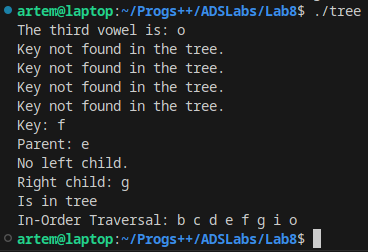
\includegraphics[width=0.90\textwidth]{Screenshot_20231108_083911.png}
    \caption{}
\end{figure}

\subsection*{Висновок} 
Бінарне дерево є структурою даних призначеною для швидкої вставки і пошуку,
всі ці операції займають $O(\log n)$. Якщо порівнювати з масивом, то в нього вставка
може бути O(n), але є можливість доступу по індексу O(1), тобто бінарне дерево в середньому краще, якщо
потрібна постійна вставка.
\end{document}
